\section*{Conventions (for authors)}
Suggestion (Sz.).
Avoid using indices whenever possible.
For example, instead of writing:
``let $G$ be a graph with vertices $v_1,v_2,\ldots,v_n$''
write
``let $G$ be a graph with vertex set $V$.''
Similarly, rather than 
``let $\phi$ be a formula with free variables $x_1,\ldots,x_n$''
write ``let $\phi$ be a formula with free variables $X$''.
The reason is that using indices leads to nested inidices, while using sets only leads to subsets.



\section{Preliminaries on graphs}
In this section, we recall some basic definitions from graphs.

% A \emph{digraph} $G$ is a pair consisting  of a set of \emph{vertices} $V$ and a set of \emph{edges} $E\subset V\times V$.
% Often, we will write $G=(V,E)$,
% and we will use the notation $V( G)$ to denote the set of vertices of $ G$
% and $E( G)$ to denote its edge set. If $(v,w)\in E( G)$, we can simply say that $vw$ is an edge of $ G$; we then call $v$ its \emph{source} and $w$ its \emph{target}.
% A \emph{self-loop} is an edge whose source and target coincide.
A \emph{graph} $G$ is a pair consisting of a set of 
\emph{vertices} $V$ and a set of \emph{edges} $E$, where each edge is a two-element subset of $V$.
Often, we will write $G=(V,E)$,
and we will use the notation $V(G)$ to denote the set of vertices of $G$
and $E(G)$ to denote its edge set. An example graph is depicted in Figure~\ref{fig:graph} below. 


\begin{figure}[h]
  \centering
	    \includegraphics[scale=0.35,page=8]{pictures.pdf}
  \caption{A graph with 9 vertices and 13 edges.}
  \label{fig:graph}
\end{figure}


The \emph{size} of a graph $G$ is $|V(G)|$.
If $e=\set{v,w}\in E(G)$, we can also write that $vw$ is an edge of $G$. We then say that $e$ is \emph{adjacent} to, or \emph{connects}, $v$ and $w$.
We also say  that $v$ and $w$ are the \emph{endpoints} of the edge $vw$.
Two vertices $v,w\in V(G)$ are \emph{neighbors} in $G$
if $vw\in E(G)$. The \emph{degree} of a vertex $v$ in $G$
is the number of its neighbors. A graph is $d$-\emph{regular} if every its vertex has degree $d$.
A graph $G$ is a \emph{clique} if any two of its distinct vertices are neighbors, and is \emph{bipartite} if there is a partition 
of its vertex set $V=V(G)$ into disjoint sets $V_1,V_2$
(called the \emph{parts}) with $V=V_1\cup V_2$, such that there are no edges in $G$ with both endpoints in the same part, i.e., all edges have one endpoint in $V_1$ and one endpoint in $V_2$. For $m,n\in\N$, by
 $K_n$ we denote the clique with vertices $\set{1,\ldots,n}$, and by $K_{m,n}$ we denote the \emph{complete bipartite graph} with $m$
 vertices in one part and $n$ vertices in the other part, with all vertices from one side connected to all vertices to the other,
 as depicted to the left in Figure~\ref{fig:bipartite} in the case $m=3,n=6$.

\begin{figure}[h]
  \centering
    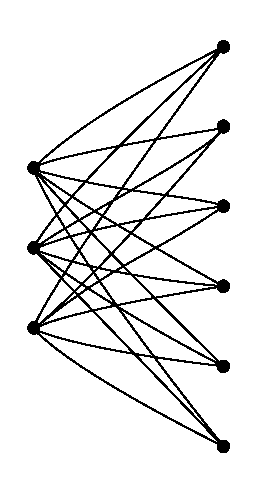
\includegraphics[scale=0.45,page=1]{pictures.pdf}\hspace{2cm}
	    \includegraphics[scale=0.45,page=2]{pictures.pdf}
  \caption{\emph{Left:} Complete bipartite graph $K_{3,6}$. \emph{Right:} The ladder $L_5$.}
  \label{fig:bipartite}
\end{figure}

\begin{example}
	An important role in stability theory is played by what we call \emph{ladder} graphs, defined as follows.
	Fix a number $k\in\N$. The \emph{$k$-ladder} is 
	the bipartite graph denoted $L_k$, with vertex set $V=\set{1,\ldots,k}\times \set{L,R}$ and edge set $E=\setof{\set{(i,L),(j,R)}}{
	1\le i\le j\le k}$. We call the sets $\set{1\ldots,k}\times \set{L}$ and $\set{1,\ldots,k}\times \set R$ the \emph{sides} of the ladder.
  The ladder $L_5$ is depicted to the right in Figure~\ref{fig:bipartite}.	
\end{example}

\begin{example}
  Another family of graphs are the \emph{powerset} graphs,
  defined as follows.
  Let $k\in\N$ be a number, and let $X=\set{1,\ldots,n}$.
  The \emph{$k$-powerset graph} is the bipartite graph denoted $P_k$, with parts $X$ and $P(X)$, 
  and edge set $E=\setof{\set{x,Y}}{x\in X,\ Y\in P(X),\ x\in Y}$. In other words, for every subset $Y$ of part $X$ of the graph there is precisely one vertex of the part $P(X)$
  which is connected to all vertices in $Y$ and to no vertices in $X-Y$.
\end{example}



Let $v,w\in V(G)$.
A \emph{walk} in $G$ is a sequence of vertices $v_0,v_1,\ldots,v_n$
such that  $v_iv_{i+1}$ is an edge in $G$ for $i=0..n-1$. This is a walk
from  $v$ to $w$ (or between $v$ and $w$) if $v=v_0$ and $v_n=v$, and has length $n$.
A \emph{path} is a walk with no repeating vertices.
The \emph{distance} between $v$ to $w$, denoted $\dist(v,w)$, is the length of a shortest walk from $v$ to $w$ (and $\infty$ if there are none). By $N_r^G(v)$ we denote the 
$r$-\emph{neighborhood} of $v$ in $G$, i.e., the
set of vertices of $G$ 
whose distance from $v$ is at most $r$. Often we will omit $G$ in the superscript when it will be understood from the context.
A graph $G$ is \emph{connected} if for every pair of its vertices, there is a walk between them.
The \emph{radius} of a graph $G$ is the smallest number $d\in\N$ such that there is a vertex $x$ with $N^G_d(x)=V(G)$.
 
A graph $G$ is \emph{planar} if, intuitively, it can be depicted on the plane $\R^2$ so that its edges do not intersect, except for perhaps 
at their endpoints\footnote{\label{ft:planar}A formal definition of planarity would require the existence a 
function $f$ (called a planar embedding of $G$) mapping each vertex  $v$ of $G$ to a points $f(v)\in\R^2$, and each 
edge $vw$ of $G$
to a continuous curve  $f(vw)\subset\R^2$ joining $f(v)$ with $f(w)$, so 
that two curves $f(e_1),f(e_2)$ associated to distinct 
edges $e_1,e_2$ intersect only perhaps at the endpoints. Here, by \emph{curve} $\Gamma$ we mean
 the image  of a continuous 1-1 function $\gamma:[0,1]\to\R^2$,
 and by the endpoints of $\Gamma$ we mean $\gamma(0)$ and $\gamma(1)$.
 One can prove that requiring the function to be 
 differentiable, or piecewise-linear, or even linear, would not affect the definition of a planar graph.}.


\paragraph{Representing graphs and algorithms}
We will use two standard data structures for representing graphs,
namely the \emph{adjacency matrix} representation and \emph{adjacency list} representation. Both representations assume an implicit linear ordering of the given graph.
We note that one can be computed from the other in polynomial time, and that the size of each representation is polynomial in terms of the number of vertices of the graph.
We will therefore take the liberty to say that an algorithm 
takes as input a graph $G$ and runs in time polynomial in $G$,
meaning that it takes as input either of the two representations of $G$
and runs in time polynomial in $|V(G)|$. 


%
%
%
%  In both representations, we assume an implicit linear ordering of the vertices of a given graph.
%  Let $G$ be a graph with $|V(G)|=n$ and $V=\set{v_1,\ldots,v_n}$.
%  Let $\#,\$\not\in\set{0,1}$ be two separator symbols.
%  The \emph{adjacency matrix} representation of  $G$
%  consists of the string $\text{bin}(n)\# w$, where
%  $\text{bin}(n)\in\set{0,1}^*$ is the binary representation
%  of $n=|V(G)|$, and $w\in\set{0,1}^*$ is the word of length $n^2$ whose  $m$th bit (where $m\in\set{0,\ldots,n^2-1}$) is set to $1$ precisely if $v_iv_j\in E(G)$, where $i,j\in\set{0,\ldots,n-1}$ are such that $m=i\cdot n+j$.
%
% The \emph{adjacency list} representation of the graph $G$
% consists of the word $\text{bin}(n)\#w_1,\#, w_2 \#,\ldots \# w_n,$
% where $w_i$ is the concatenation of all
 



% Sometimes, when we will want to underline the fact that something is a digraph rather than a graph, we will denote it by $\di G$. Many definitions below
% apply to both graphs and digraphs, so $G=(V,E)$ might denote them.

% Fix a set $C$ of \emph{colors}.
% A \emph{colored graph} (colored by $C$)
% is a graph $G$ together with a function $\col:V(G)\to C$, assigning a color $\col(v)$ to each vertex  $v\in V(G)$.

\paragraph{Subgraphs, embeddings, isomorphisms}
If $G$ is a graph, then a \emph{subgraph} of $G$
is a graph $H$ such that $V(H)\subset V(G)$
and $E(H)\subset E(G)$. We say that $H$
is an \emph{induced} subgraph of $G$
if $E(H)=E(G)\cap (V(H)\times V(H))$.
The subgraph of $G$ induced by a set vertices $W\subset V(G)$ is the graph denoted $G[W]$ with vertices $W$ and edge set $E(G)\cap (W\times W)$. 

If $H$ and $G$ are graphs, then an \emph{embedding}
of $H$ into $G$ is a 1-1 function $f:V(H)\to V(G)$
such that for every pair $v,w\in V$, 
$vw$ is an edge of $H$ if and only if $f(v)f(w)$ is an edge of $G$. 
We write $f:H\to G$ when $f$ is an embedding of $H$ into $G$.
We say that $H$ \emph{embeds} into $G$ if there is an embedding of $H$ into $G$.
An \emph{isomorphism} is a surjective embedding.  Note that $H$ embeds into $G$ if and only if $H$ is isomorphic to an induced subgraph of~$G$.


\paragraph{Minors}
Let $G$ and $H$ be two graphs.
% Fix a number $d\in\N$.
A \emph{minor model} of $H$ in $G$
is a mapping $B$
which maps each vertex $v$ of $H$ to a connected subgraph $B(v)$ of $G$,
called the \emph{bag} of $v$,
and each edge $vw$ of $H$ to an edge $B(vw)$ of $G$,
subject to the following conditions
(cf. Figure~\ref{fig:minor}):
 % such that for all $v,w\in V(G)$ the following conditions hold:
\begin{itemize}
	\item Bags of distinct vertices are pairwise disjoint, i.e.,  $V(B(v))\cap V(B(w))=\emptyset$ for all
	 $v,w\in V(H)$ such that $v\neq w$;
	\item For every edge $vw\in E(H)$, the edge $B(vw)$ joins a vertex in $V(B(v))$ with a vertex in $V(B(w))$.
\end{itemize}



\begin{figure}[h]
  \centering
    \includegraphics[scale=0.35,page=6]{pictures.pdf}
  \caption{The graph $H$ depicted above is a minor (at depth $1$) of the graph $G$. The minor model maps a vertex $v$ of $H$ to the subgraph $B(v)$ of $G$ induced by the spot of the same color as $v$,
  and maps an edge $vw$ to the thick edge joining $B(v)$ with $B(w)$.
  }
   \label{fig:minor}
\end{figure}

We say that $H$ is a \emph{minor} of $G$
if there is a minor model of $H$ in $G$. 
The \emph{radius} of a minor 
model is the maximal radius of all of its bags.
If $d\in\N$,
we say that $H$ is a minor of $G$
at \emph{depth} $d$ if there is a minor model of $H$
in $G$ of radius $d$.

\paragraph{Conventions}
Often, the 
behavior of the function
 $B$ on edges will be irrelevant, and it will only matter that 
 for every edge $vw\in E(H)$ there is some edge joining a vertex in $V(B(v))$ with a vertex $V(B(w))$. In this case, the model $B$ can be 
 described by providing its behavior on vertices (i.e, the bags associated to each vertex), and the extension to edges can be chosen arbitrarily. Also, since adding or removing edges to a bag $B(v)$ cannot 
 spoil the model $B$ as long as the bag remains connected, in many cases, we may simply provide the vertex set $W\subset V(G)$ of the bag of $v$, and assume that $B(v)=G[W]$ is the subgraph of $G$ induced by $W$.
 On the other extreme,  
 we may always modify a minor model (without altering its radius) so that each bag is a spanning tree; in this case, we will say that $B$ is a minor model whose bags are trees. 
 


\paragraph{Topological minors}
A \emph{topological minor model} of $H$ in $G$
is a mapping $M$ 
mapping vertices of $H$ to vertices of $G$ 
and  edges of $H$ to paths in $G$,
subject to the following conditions:
\begin{itemize}
	\item For every edge $vw\in E(H)$, 
	$M(vw)$ is a path from $M(v)$ to $M(w)$ in $G$,
	\item For every pair of edges $e,f\in E(H)$,
	the paths $M(e)$ and $M(f)$ have no common vertices,
	except for perhaps their endpoints.	
\end{itemize}
Since the behavior of $M$ on vertices can be deduced from the behavior on edges, we will often describe $M$ by simply providing the latter.

We say that $H$ is a \emph{topological minor} of $G$
if there is a topological minor model of $H$ in $G$.
If $d\in \N$, we say that $H$ is a topological minor of $G$ at \emph{depth} $d$ if there is a topological minor model $M$ of $H$ in $G$ with the property that 
$M(vw)$ is a path of length at most $d+1$, for each edge $vw\in E(H)$.


\begin{figure}[h]
  \centering
    \includegraphics[scale=0.35,page=7]{pictures.pdf}
  \caption{The graph $H$ depicted above is a topological minor (at depth $2$) of the graph $G$. The minor model maps a vertex $v$ of $H$ to the vertex of $G$ with the same color, and edges of $H$ to the   paths in $G$ delineated using thick edges.} 
  % \label{fig:bipartite}
\end{figure}

\begin{example}
	Let $G_{k\times k}$ denote the $k\times k$ grid, depicted  in 
	Figure~\ref{fig:grid} to the left, in the case $k=5$. Then every planar 
	graph 
	is a minor of $G_{k\times k}$, for sufficiently large $k$.
	This is illustrated in Figure~\ref{fig:grid}, to the right.
	However, the star with five arms, which is clearly planar, is not a topological minor of any grid $G_{k\times k}$, since it has a vertex of degree $5$, while $G_{k\times k}$ has  vertices of degree at most $4$,
	and topological minors cannot increase the maximal degree.
	
	
	\begin{figure}[h]
	  \centering
	    \includegraphics[scale=0.35,page=5]{pictures.pdf}\hspace{3cm}
	    \includegraphics[scale=0.35,page=9]{pictures.pdf}		
	  \caption{\emph{Left:} The $5\times 5$ grid.
	  \emph{Right:} The planar graph $H$ is a minor of the grid $G_{k\times k}$,
	  for some large $k$.
	  } 
	  \label{fig:grid}
	\end{figure}	

\end{example}

\begin{example}\label{ex:topminor-minor}
	If $H$ is a topological minor of $G$ then $H$ is also a minor of $G$.
	More precisely, if $H$ is a topological minor of $G$ at depth $d$,
	then $H$ is a minor of $G$ at depth $\lceil d/2 \rceil$.
	Indeed -- a topological minor model $M$ of $H$ in $G$
	can be converted into a minor model $B$ of $H$ in $G$, as follows.
	For each edge $vw\in E(H)$, consider the path $M(vw)$ joining $M(v)$
	with $M(w)$. Distribute the vertices along this path, by assigning a vertex $w\in M(vw)$ 
	to either $B(v)$ or $B(w)$, depending on whether its is closer to $M(v)$
	or to $M(w)$ along the path (in case of a tie, choose arbitrarily).
	Note that the vertices added to $B(v)$ have distance at most $\lceil d/2\rceil$ to $M(v)$.
	By repeating this for each edge $e$ in $E(H)$, we have constructed a set $B(v)$, for each $v\in V(H)$. We identify this set with the subgraph of $G$ which it induces. Then $B$ is a graph minor model of $H$ in $G$.
\end{example}

\begin{lemma}\label{lem:minor-transitivity}
  If $G_1\in\minors {d_1} {G_2}$ and $G_2\in\minors {d_2} {G_3}$,
  then $G_1\in\minors d {G_3}$, where $d=\ldots$.
  Similarly, 
  if $G_1\in\tminors {d_1} {G_2}$ and $G_2\in\tminors {d_2} {G_3}$,
  then $G_1\in\tminors d {G_3}$, where $d=\ldots$.
\end{lemma}



\paragraph{Subdivisions}
If $G=(V,E)$ is a graph and $e$ is its edge,
then \emph{subdividing} this edge  $k$ times results in replacing the edge $e$
by a path of length $k+1$, as depicted to the left in Figure~\ref{fig:subdivision} in the case $k=2$.


\begin{figure}[h]
  \centering
    \includegraphics[scale=0.35,page=3]{pictures.pdf}\hspace{2cm}    \includegraphics[scale=0.35,page=4]{pictures.pdf}
  \caption{\emph{Left:} The process of subdividing an edge two times.
  \emph{Right:} The maximal 1-subdivision of $K_5$.
  } 
  \label{fig:subdivision}
\end{figure}


A $k$-\emph{subdivision} of the graph $G$
is any graph obtained by subdividing each of its edges
at most $k$ times. The vertices of the original graph $G$
are called the \emph{principal} vertices of the resulting subdivided graph.
The \emph{maximal} $k$-subdivision of $G$ is obtained by subdividing each edge of $G$ exactly $k$ times. The maximal $1$-subdivision of $K_5$
is depicted in  Figure~\ref{fig:subdivision}, to the right.




The following lemma relates subdivisions to topological minors.
\begin{lemma}\label{lem:minors-subdivisions}
  Let $H,G$  be graphs. Then
  	$H$ is a topological minor of $G$ at depth $d$
  	if and only if some $d$-subdivision of $H$
  	is isomorphic to a subgraph of $G$.
\end{lemma}


\paragraph{Graph congruences}
Let $G$ be a graph and let $\sim$ be an equivalence relation on $V(G)$. Then $\sim$ is a \emph{congruence} of $G$ if 
whenever $v_1,w_1,v_2,w_2\in V(G)$ are such that 
 $v_1\sim v_2$ and $w_1\sim w_2$, then $v_1w_1\in E(G)$ if and only if $v_2w_2\in E(G)$. In other words,
  for any two equivalence classes $c,d\in V(G)/{\sim}$, the graph $G[c\cup d]$ is either a complete bipartite graph with parts $c,d$, or has no edges. In particular, taking  $c=d$, we see that $G[c]$ has no edges for each equivalence class $c$.
 We denote by $G/{\sim}$ the quotient graph,
 with vertex set $V(G)/{\sim}$, in which two equivalence classes $c,d\in V(G)/{\sim}$ are adjacent precisely when $G[c\cup d]$ is the complete bipartite graph with parts $c,d$. Observe that the quotient graph $G/{\sim}$ is isomorphic to an induced subgraph of $G$: if  $f:V(G/{\sim})\to V(G)$ is any mapping which maps an equivalence class $c\in V(G)$ to any of its elements, then $f$ is an embedding of $G/\sim$ into $G$.
 
 

\section{Preliminaries on logic}
In this section, we recall some basic definitions from logic. We start from defining relations, which we call here {tables} for brevity.



\paragraph{Tuples and tables}
Let $X$ and $Y$ be two sets.
We will sometimes call a function from $X$ to $Y$
a \emph{tuple over $X$}, or \emph{indexed by} $X$, with \emph{values from} $Y$. 
If we omit the set $Y$ from this notation, and 
just talk about a tuple over $X$, then~$Y$ is allowed to be an arbitrary set. 
If $t$ is a tuple over $X$ and $U\subset X$, then
by $t[U]$ we denote the tuple obtained from restricting the tuple $t$ to $U$. For $x\in X$ we will also write $t[x]$ to denote $t(x)$, and call $t[x]$ the \emph{value} of $t$ at \emph{position} $x$.
We also say that $t[x]$ is an \emph{element} of the tuple $t$.
For defining tuples, we may use the $\mapsto$ notation, e.g., $\set{x\mapsto 1,y\mapsto 2}$
denotes the tuple $t$ such that $t[x]=1$ and $t[y]=2$.
If $n\in\N$, then an \emph{$n$-tuple} $t$ is a tuple over $\set{1,\ldots,n}$. The tuple $\set{1\mapsto y_1,\ldots,n\mapsto y_n}$ can be also denoted $(y_1,\ldots,y_n)$. We may also simply that $y_1,\ldots,y_n$ is a tuple of elements.
The \emph{empty tuple}, denoted $\eps$, is the unique tuple $\eps:\emptyset\to\emptyset$ indexed by $\emptyset$.



If $t$ is a tuple over $X$ with values from $Y$,
and $f:Y\to Y'$ is a function, then by $f(t)$
we denote the tuple over $X$ with values from $Y'$ obtained by applying $f$ element-wise, i.e., $f(t)[x]=f(t[x])$ for $x\in X$.

A \emph{table over} $X$ (with values from $Y$) is a set of tuples over $X$ (with values from $Y$).
If $T$ is such a table and $U\subset X$, then by 
$T[U]$ we denote the set of all tuples $t[U]$, for $t\in T$.
There are two tables over $\emptyset$: the empty table, and the table consisting of the empty tuple $\eps$.

% If $Y$ is a set, then  $\Fun X Y$ denotes the table consisting of all tuples over $X$ with values from $Y$.





\paragraph{First-order logic}
Fix an infinite, countable set of \emph{variables} $\Vv=\set{x,y,\ldots}$.
We inductively define the syntax  of \emph{formulas} for graphs.
Every formula $\phi$ will additionally have an associated set of \emph{free variables}
$\fv(\phi)\subset \Vv$.

\begin{itemize}
	\item $\top$ and $\bot$ are formulas with no free variables.
	\item If $x,y$ are variables then $x=y$ and $xy\in E$ are formulas. For each of them, the set of free variables is $\set{x,y}$.
	\item If $\phi,\psi$ are formulas, then $\phi\land \psi,\phi\lor\psi,\phi\implies\psi,\phi\iff\psi$ are formulas with free variables $\fv(\phi)\cup\fv(\psi)$, and $\neg\phi$ is a formula with free variables $\fv(\phi)$.	
	
	\item If $\phi$ is a formula and $x$ is a variable then $\forall x.\phi$ and $\exists x. \phi$ are formulas, whose set of free variables is $\fv(\phi)-\set x$.
\end{itemize}



The semantics of formulas is also defined by induction.
Fix a graph $G=(V,E)$. 
% If $X$ is a set of variables, then a \emph{valuation} of $X$ in $G$ is a function $\val :X\to V$. We also write $\val \in V^X$.
For a formula $\phi$ with free variables $X$ we inductively define its \emph{semantics} in $G$, denoted $\sem \phi_G$, which is a table
over $X$ with values from $V$, i.e., $\sem \phi_G\subset (\Fun X V)$:
\begin{itemize}
	\item If $\phi$ is $\top$, then 
	$\sem \phi_G$ is the table $\set{\eps}$ over $\emptyset$ consisting only of the empty tuple $\eps$.
	
	\item If $\phi$ is $\bot$, then 
	$\sem \phi_G$ is the empty table over $\emptyset$.	
	
	\item If $\phi$ is of the form $x=y$, then
	$\sem \phi_G$ consists of all those tuples $\fun \val {\set {x,y}} V$,
	such that $\val[x]=\val[y].$

	\item If $\phi$ is of the form $xy\in E$, then
	$\sem \phi_G$ consists of all those tuples $\fun \val {\set {x,y}} V$,
	such that $\val[x]\val[y]\in E.$
		
	\item If $\phi$ is of the form $\exists x.\psi$, then
	$\sem \psi_G=\sem \phi_G[\fv(\phi)].$ In other words,
	$\sem\psi_G$ consists of those tuples $s$ over $\fv(\phi)$, which extend to some tuple $t$ over $\fv(\psi)$ such that $t\in \sem \psi_G$.
	
	\item If $\phi$ is of the form $\psi\lor \gamma$, then $\sem \phi_G$
	is defined as the set of those tuples $\fun\val {\fv(\psi)\cup\fv(\phi)} V$,
	such that $\val[{\fv(\phi)}]\in \sem \phi_G$ or $\val[{\fv(\psi)}]\in \sem \psi_G$ (or both).
	
	\item If $\phi$ is of the form $\neg\psi$, then $\sem\phi_G=(\Fun {\fv(\psi)} V) - \sem\psi_G$, i.e., 
	$\sem \phi_G$ consists of all tuples $t$ over $\fv(\psi)=\fv(\phi)$ such that $t$ does not belong to $\sem\psi_G$.
	

\item The semantics for $\forall x.\phi$ is defined as the semantics of $\neg\exists x.\neg\phi$, and the semantics of $\phi\land \psi,\phi\implies\psi,\phi\iff\psi$ is defined as usual using $\lor$ and $\neg$.
\end{itemize}


This finishes the definition of formulas of first-order logic for graphs. In this paper, when we say \emph{formula} we implicitly mean such a formula, unless stated otherwise.
A formula $\phi$ with no free variables is called a \emph{sentence}. The variables which occur in a formula, but are not free are called \emph{bound} variables.
The \emph{size} of a formula is the number of symbols it consists of.
Note that there are finitely many formulas of a fixed size.
Two formulas $\phi, \psi$ with $\fv(\phi)=\fv(\psi)$ are \emph{equivalent} if for any (finite or infinite) graph $G$, $\sem\phi_G=\sem\psi_G$.
Note that $\top$ 
is equivalent to $\forall x.x=x$, $\bot$ is equivalent to $\exists x.\neg (x= x)$,
so the formulas $\bot$ and $\top$, as well as the constructs 
$\land,\implies,\iff,\forall$
 are (up to equivalence) redundant in our definition of first-order logic, and in the inductive proofs it is enough to assume that formulas do not use these constructs, and use only the constructs $x=y, xy\in E$
 (called the \emph{atomic} formulas) and the boolean connectives
 $\lor,\neg$.

\begin{proposition}\label{pro:fo-evaluation}
	Fix a formula $\phi$. For a given graph $G$, 
	the table $\sem\phi_G$ can be computed in time polynomial in $G$.
\end{proposition}
\begin{proof}	
	The proof proceeds by induction on the structure of the formula $\phi$. We  represent tables in the standard way, as arrays.
	The base case consists of the atomic formulas $xy\in E,x=y$, for which the claim holds, assuming either the adjacency matrix or adjacency list representation of the input graph $G$. In the inductive step, when $\phi$ is of one of the forms $\exists x.\psi,\ \psi\lor\gamma$, or $\neg \psi$, we observe that the definition of the semantics gives a naive evaluation algorithm of $\sem\phi_G$ from $\sem\psi_G$ and $\sem \gamma_G$.
\end{proof}


\paragraph{Conventions}
If $\cal F$ is a finite set of formulas, then we may write 
$\bigvee \cal F$ to denote $\phi_{1}\lor \phi_{2}\lor\ldots \phi_{n}$, where $\phi_1,\ldots,\phi_n$ is an enumeration of $\cal F$ in any order. Similarly, 
if $\family{\phi_i}{i\in I}$ is a finite family of formulas, then  $\bigvee_{i\in I} \phi_i$ denotes
$\bigvee \setof{\phi_i}{i\in I}$. This convention applies also to $\bigwedge$ in place of~$\bigvee$.
Also, we will often write $\exists x_1\ldots x_n.\phi$ as  shorthand for $\exists x_1.\exists x_2\ldots\exists x_n.\phi$.
We use $x\neq y$ as shorthand for $\neg (x=y)$.

When $\val\in\sem \phi_G$, we may also say that $\val$ \emph{satisfies}
the formula $\phi$ in~$G$. We may also skip the graph $G$,
if it is understood from the context.
 If $\phi$ is a formula with 
free variables $X$, and an assignment $t$ of some vertices
$v_1,\ldots,v_n\in V(G)$  to $X$ is implicit,
then we may say that $v_1,\ldots,v_n$ 
satisfies the formula $\phi$, whenever  $t$ satisfies $\phi$ in $G$. In particular, if $X=\set x$ is a singleton, 
then we will often say that $v\in V(G)$ satisfies $\phi$,
meaning that  $t\in \sem \phi_G$, where $t:X\to V(G)$ is  such that $t[x]=v$. In the extreme case when
$\phi$ is a sentence and $X=\fv(\phi)=\emptyset$, then $\sem \phi_G$
is a subset of $\set\varepsilon$, where $\varepsilon$
is the {empty tuple}. In particular, $\sem\phi_G$ is either empty  or $\sem\phi_G=\set\varepsilon$. In the latter case we say that $\phi$ is satisfied in $G$, or $\phi$ holds in $G$. 

Any formula $\phi$ with free variables $X$ can be treated as a formula with free variables $Y$, for a set $Y$ containing $X$: it is enough to replace $\phi$
by the formula $\phi\land \bigwedge_{y\in Y}(y=y)$.
Therefore, in the sequel, when saying $\phi$
\emph{is a formula with free variables} $Y$, we will actually also allow $\phi$ to be a formula with $\fv(\phi)\subset Y$. 
We may write $\phi(x,\ldots,z)$ 
to indicate that $\phi$ is treated as a formula with free variables $x,\ldots,z$. For instance, we may write
$\phi(x,y)=\top$, which means that $\phi$ is the formula with free variables $x,y$, obtained from $\top$ as described above,
i.e., $\phi=\top\land(x=x)\land (y=y)$.

If $\phi$ is a formula and $s:\fv(\phi)\to\Vv$ is a function, then by $\phi\, s$ we denote the formula 
$\psi$ obtained by substituting the free variables of $\phi$
according to $s$. For example, 
If $\phi$ is the formula $xy\in E$ then $\phi\, \set{x\mapsto p,y\mapsto r}$ is the formula $pr\in E$.
One has to be careful when substituting the free variables:
 first rename all bound variables in $\phi$
by fresh variables (i.e., not appearing in $\phi$ nor in~$s$), and then rename the free variables according to $s$. For example, if $\phi$ is the formula $\exists y.xy\in E$ then $\phi\,\set{x\mapsto y}$ is the formula $\exists z.yz\in E$, where $z$ is some fresh variable.


Finally, whenever $\textit{desc}$ is any mathematical description of a property
(using words, formulas, or their combination) of some elements $x,\ldots,z$ which is known to be definable by some  first-order formula $\phi(x,\ldots,z)$, then by $[desc]$ we mean the formula $\phi$.
For instance, we will show in Example~\ref{ex:dist} 
that for any fixed $d\in \N$ there is a first-order formula $\phi(x,y)$ expressing the property 
``$x$ and $y$ are at distance at most $d$'', i.e., $\dist(x,y)\le d$. Then $[\dist(x,y)\le d]$ is shorthand for the formula $\phi$.




\begin{example}\label{ex:walk}
	Let $\phi$ be the formula $$\exists x_0.\exists x_1.\exists x_2.\exists x_3.(x=x_0)\land (x_0x_1\in E)\land (x_1x_2\in E)\land (x_2x_3\in E)\land (x_3=y),$$
	which can be also written as $\exists x_0\ldots x_3. (x=x_0)\land (x_3=y)\land\bigwedge_{i=0..2} (x_ix_{i+1}\in E)$. Then $\fv(\phi)=\set{x,y}$.
	For a graph $G=(V,E)$, the set $\sem \phi_G$ consists of all tuples
	$\set{x\mapsto v,y\mapsto w}$ such that $v,w\in V$ and there is a walk from $v$ to $w$
	of length exactly $3$. For each such a tuple, we may also say that the pair of vertices $v,w\in V(G)$ satisfies $\phi$.
\end{example}
	
\begin{example}\label{ex:dist}
	In a similar way, we may write a first-order formula 
	$\phi^d$ expressing the property that $\dist(x,y)\le d$, for a fixed value $d\in\N$:
	$$\phi^d\ =\bigvee_{d=0..r}\left(\exists x_0\ldots x_r. (x=x_0)\land (x_r=y)\land\bigwedge_{i=0..d} (x_ix_{i+1}\in E)\right).$$ 
\end{example}	

\begin{example}\label{ex:deg}
	For a fixed $k\in\N$, the  formula $$\delta_{\ge k}\ =\ \exists x_1\ldots x_k \bigwedge_{1\le i<j\le k} \neg(x_i=x_j)\land \bigwedge_{1\le i\le k}
	(x_ix\in E)$$ with free variable $x$ expresses the property that $x$ has degree at least $k$.
	The formula $\delta_{\ge k}\land \neg\delta_{\ge {k+1}}$ expresses the property that $x$ has degree exactly $k$.
\end{example}



\begin{example}
  The following sentence $\psi$ expresses the property that
  a graph has an \emph{independent set of size $k$}:
  $$\psi=\exists x_1\ldots x_k.\bigwedge_{1\le i<j\le k}\neg[\dist(x_i,x_j)\le 1].$$
  More explicitly,
$$\psi=\exists x_1\ldots x_k.\bigwedge_{1\le i<j\le k}\neg((x_i=x_j)\lor (x_ix_j\in E)).$$

	The following sentence $\phi$ expresses the property that a graph has \emph{a dominating set of size $k$}:
  $$\phi=\exists x_1\ldots x_k.\forall x.\bigvee_{i=1..k}[\dist(x,x_i)\le 1].$$
  More explicitly,
  $$\phi=\exists x_1\ldots x_k.\forall x.\bigvee_{i=1..k}
  (x=x_i)\lor (xx_i\in E).$$
\end{example}

\begin{example}\label{ex:ladder}
  This example shows that using a fixed formula $\phi(x,y)$, one can define a partial order $\leqslant$
  on the vertices of the ladder $L_k$, 
  so that for two vertices $v,w\in V(L_k)$,
  $v\leqslant w$ if and only if $v$ and $w$
  are on the same side of the ladder, and $\deg(v)\le \deg(w)$ (see Figure~\ref{fig:ladder-order}).
  \begin{figure}[h]
    \centering
      \includegraphics[scale=0.35,page=14]{pictures}
    \caption{The ordering of the ladder.}
    \label{fig:ladder-order}
  \end{figure}
    Note that the degrees of the vertices on one side of the ladder are $1,2,\ldots,k$; in particular, they are unbounded, for unbounded $k\in\N$, so it is not immediately clear how to order the vertices according to the degree using a fixed formula. However, observe that 
    in the ladder $L_k$,
    if $x,y$ are two vertices on the same side of the ladder,
    then $\deg(x)\le \deg(y)$ if and only if $N_1(x)\subset N_2(y)$. The property $N_1(x)\subset N_2(y)$ is defined by the following formula:
  \begin{align*}
    \phi(x,y)&=\forall z.(xz\in E)\implies (yz\in E).
  \end{align*}
Hence, $\phi(x,y)$ if and only if $x\leqslant y$.

We now define a formula $\psi(x,y)$ which defines a bijection between the two sides of the ladder $L_k$,
which matches every vertex on one side with the corresponding vertex on the other side. The formula $\psi(x,y)$
expresses the property: $y$ is the smallest neighbor of $x$,
with respect to the linear order defined by $\phi$:
\begin{align*}
  \psi(x,y)&=(xy\in E)\land \forall z.\big((xz\in E)\implies(\phi\,\set{x\mapsto y,y\mapsto z})\big).
\end{align*}
\end{example}



\paragraph{Locality}
In this section, we recall the notion of Gaifman locality for first-order logic. 
Fix a graph $G$ and a number $d\in\N$. Let $t$ be a tuple over a set $X$, consisting of vertices of $G$.
By $N_d(t)$ we denote the subgraph of $G$ induced by the set of vertices of distance at most $d$ from some element of the tuple $t$.
If $t,s$ are two such tuples, we say that they have \emph{isomorphic} 
$d$-neighborhoods if there is an isomorphism  $f:N_d(t)\to N_d(s)$
which maps $t$ to $s$, i.e., $f(t)=s$. 
A $d$-\emph{neighborhood type} over $X$ is an equivalence class
of the relation of having isomorphic $d$-neighborhoods. 
A $d$-neighborhood type over $X$ can be represented by a graph $T$, together
with a distinguished tuple of vertices $t$ indexed by $X$, i.e.,
$t:X\to V(T)$, with the property that $N_d(t)=T$.
\sz{pic of $d$-neighborhood type}

We say that a formula $\phi$ is \emph{$d$-local} if for every graph $G$
and for every two tuples $s,t$ over $\fv(\phi)$ with isomorphic $d$-neighborhoods, 
either both $s,t$ belong to $\sem\phi_G$, or both $s,t$ do not belong to $\sem\phi_G$. In other words, whether a tuple $t$ of vertices of $G$ satisfies $\phi$ depends only on the $d$-neighborhood type of  the tuple $t$ (as well as of global properties of $G$, independent on the choice of the tuple $t$).

\begin{theorem}[Gaifman's locality]\label{thm:gaifman}
	Let $\phi$ be a formula of first-order logic for graphs.
	Then there is a number $d\in\N$ such that $\phi$ is $d$-local.	
	Moreover, the number $d$ can be computed from $\phi$.
\end{theorem}

\sz{Perhaps the theorem about Gaifman normal form would be more useful}
\begin{example}
	For $n\in\N$, let $P_n$ denote the graph with vertices $v_0,\ldots,v_n$ whose edges are pairs $v_{i}v_{i-1}$, for $i=1,\ldots,{n}$. 
	The graph $P_n$ is called the \emph{path} of length $n$; the vertices $v_0$ and $v_n$ are called the endpoints. There is a formula $\phi(x)$ such that a vertex $v\in V(P_n)$ satisfies $\phi$ if and only if $v$ is an endpoint -- indeed, it suffices to take the formula $\neg\delta_{\ge 2}$ from Example~\ref{ex:deg}. There is no formula $\psi(x)$
	such that $v\in V(P_n)$ satisfies $\psi$ if and only if $v=v_0$. Intuitively, the vertices $v_0$ and $v_n$
	of $P_n$ are indistinguishable by first-order logic. One does not even need Gaifman locality to prove this -- it is sufficient to
	 observe (and prove by induction)  that the semantics of first-order logic is preserved under isomorphism, i.e., if $s$
	and $t$ are two tuples of elements of $G$ and there is an isomorphism $f:G\to G$ which maps $s$ to $t$, then $s\in \sem\phi_G$
	if and only if $t\in \sem \phi_G$. Clearly, there is an isomorphism of $P_n$ to $P_n$ which maps $v_0$ to $v_n$.
	
		
	
	
	For each \emph{fixed} $n$  there is a formula $\textit{even}_n(x)$ such that $v\in V(P_n)$ satisfies $\textit{even}_n(x)$ if and only there is an even-length path from $v$ to one of the endpoints of $P_n$ -- it suffices to take $$\textit{even}_n(x)=	
	\bigvee_{k=0..n}
	(\exists y.
	[\deg(y)=1]\land
	[\dist(x,y)=2k]).$$
	However, the size of any  formula expressing this property necessarily depends on $n$.
	Indeed, suppose that  $\phi$ is a formula with one free variable $x$.
	% such that for all numbers $m,n\in N$ such that $m\le 2n$,
	%  $v_m$ satisfies $\phi$ in $P_{2n}$ if and only if $m$ is even.
	 Let $d$ be the number from Gaifman's locality theorem. 
	 Then for any $k,l,n\in \N$ such that $d< k,l< n-d$,
	 the $d$-neighborhoods of $v_k$ and of $v_l$
	 are isomorphic in $G$, so	 
	 whenever $v_k$ satisfies $\phi$, 
	 also $v_l$ satisfies $\phi$.
\end{example}


% \paragraph{First-order logic for digraphs, colored graphs, colored digraphs}
% The above definition of first-order logic can be applied verbatim to
% digraphs. We can also define first-order logic for colored (di)graphs.
% The definitions of syntax and semantics extend the above definitions, by
% allowing a new formula $\col(x)=c$ for
% each fixed color $c\in C$ and variable $x\in \Vv$. Its set of free variables
% is $\set x$ only (without $c$, since $c$ is fixed).
% Furthermore, for a fixed colored (di)graph $G$ (with an implicit coloring $\col:V(G)\to C$)
% we define the semantics $\sem \phi_G$ of such a formula $\phi$ as the set of those tuples $\val:\set x\to V$ which map $x$
% to a vertex of color $c$ in $V$, i.e., $\col(\val(x))$.

\paragraph{Interpretations}
We now describe how formulas can define new graphs out of old ones. Roughly, the idea is that the vertices of the new graph are tuples of vertices of the old graph 
of a fixed length $d$,
and the edges of the new graph are specified by a formula with $2d$ free variables.

We will use the following notation.
For two sets $X,Y$, denote by $X\disjoint Y$
the disjoint union of $X$ and~$Y$, formally defined as $X\disjoint Y=(X\times\set{1})\cup (Y\times \set {2})$.
For an element $x\in X$, denote $x_1\eqdef (x,1)$ and for an element $y\in Y$, denote $y_2\eqdef(y,2)$.
 If $s$ is a tuple over $X$ and $t$ is a tuple over $Y$, then  $s\disjoint t$ denotes
the tuple over $X\disjoint Y$ defined in the obvious way, so that $(s\disjoint t)[x_1]=s[x]$
and $(s\disjoint t)[y_2]=t[y]$.


An \emph{interpretation} is a pair $\Phi=(\phi_V,\phi_E)$ consisting of two formulas,
$\phi_V,\phi_E$ such that if $\fv(\phi_V)=X$, then
$\fv(\phi_E)=X\disjoint X=\setof{x_1}{x\in X}\cup \setof{x_2}{x\in X}$, the disjoint union of two copies of $X$.
For a given graph $G$, define a new graph $\Phi(G)$ as follows:
\begin{align*}
V(\Phi(G))&\eqdef\sem {\phi_V}_G,&
E(\Phi(G))&\eqdef\setof{\set{s, t}}{s,t\in\sem{\phi_V}_G,\ s\neq t,\ s\disjoint t\in \sem{\phi_E}_G}.
\end{align*}
 If a graph $H$ is isomorphic to a graph $\Phi(G)$,
for some interpretation~$\Phi$, then we say that $H$ \emph{interprets} in $G$.
The \emph{dimension} of the interpretation $\Phi$
is the number of free variables of the formula $\phi_V$, i.e., $|\fv(\phi_V)|$. Note that $\Phi(G)$ has at most $|V(G)|^d$ vertices, if $\Phi$ is an interpretation of dimension $d$.

\begin{remark}
  Observe that in the interpretation $\Phi$,
  the formula $\phi_E$ might be not symmetric,
  i.e., it may be the case that $s\disjoint t\in\sem{\phi_E}_G$ while $t\disjoint s\notin\sem{\phi_E}_G$,
  or may contain self-loops, i.e., it may be the case that $s\disjoint s\in\sem{\phi_E}_G$. Nevertheless, according to the above definition, the resulting graph $\Phi(G)$ contains no self-loops and is undirected.
  It is not difficult to show that any interpretation $\Phi=(\phi_V,\phi_E)$ can be converted into an interpretation $\Phi'=(\phi_V',\phi_E')$ of the same dimension, which is equivalent to $\Phi$, i.e., 
  $\Phi(G)=\Phi'(G)$ for every graph $G$, and moreover such that $\Phi'$ is symmetric and without self-loops.  
\end{remark}




\begin{example}
	Let $\Phi=(\phi_V,\phi_E)$
	be the interpretation in which
	$\phi_V(x,y,z)=\top$, where $\fv(\phi_V)=\set{x,y,z}=:X$, and  $\phi_E$
	is the formula with free variables $X\disjoint X$
	given by:
 $$\phi_E(x_1,y_1,z_1,x_2,y_2,z_2)=
	\neg ((x_1= x_2)\land (y_1=y_2)\land(z_1=z_2)).$$
	For a given graph $G$, the graph
	$\Phi(G)$ is the clique on $|V(G)|^3$ vertices.
	More generally, observe that for any fixed interpretation $\Phi$,
	the size of $\Phi(G)$ is polynomial in the size of $G$, and $\Phi(G)$
	can be computed in polynomial time from $G$.
\end{example}

\begin{example}\label{ex:subdivision-undo}
  Fix a number $k\in \N$.
	Let $H$ be the maximal $k$-subdivision of a graph $G$
	without vertices of degree $2$; for example, $G$ may be $d$-regular, for some $d\ge 3$.
	Then $G$ interprets in $H$, via a 1-dimensional interpretation $\Phi=(\phi_V,\phi_E)$, where
	\begin{align*}
		\phi_V(x)&=\neg[\deg(x)=2]\\
		\phi_E(x_1,x_2)&=[\dist(x_1,x_2)=k+1].
	\end{align*}
  
  Now suppose that $H$ is some (not necessarily maximal) $k$-subdivision of a graph $G$ without vertices of degree 2. Then $G$ still interprets in $H$, via the interpretation $\Psi$ defined below.
  First observe that for any fixed $d\in\N$, the property ``the vertices $x,y$ 
  can be connected by a path of length at most $d$, which passes only through vertices of degree $2$''
  can be expressed by a first-order formula $\psi^d(x,y)$,
  similarly as in the formula $\phi^d$:
  it suffices to add to $\phi^d$ the conjuncts $[\deg(x_i)=2]$
  for $i=1,\ldots,r-1$.
  Define $\Psi$ as the interpretation consisting of the formula $\psi_V(x)=\neg[\deg(x)=2]$,
  and the formula $\psi_E$ obtained from $\psi^{k+1}$ by substituting the variables $x$ by $x_1$ and $y$ by $y_1$.  
\end{example}

\begin{example}
	Interpretations can act as ``filters''.
	Let $\phi$ be a sentence. Then there is an interpretation $\Phi$
	such that $\Phi(G)=G$ if $G$ satisfies $\phi$, and $\Phi(G)$
	is the empty graph otherwise. Indeed, it suffices to take
	$\phi_V(x)=\phi$ (where $x$ does not appear in $\phi$)  and $\phi_E(x_1,x_2)=x_1x_2\in E$.
\end{example}


\begin{example}\label{ex:subdivide}
Consider the following interpretation $\Phi=(\phi_V,\phi_E)$, 
where 
	\begin{align*}
		\phi_V(x,y)&=(x=y)\lor (xy\in E)\\
		\phi_E(x_1,y_1,x_2,y_2)&=([x_1=y_1=x_2]\land (x_2y_2\in E))\lor ((x_1y_1\in E)\land(x_1=y_2)\land (x_2=y_1)).
	\end{align*}
The result of applying $\Phi$ to a graph $G$ is depicted in Figure~\ref{fig:int-subdivide}. It is not difficult to see that for every graph $G$, the graph $\Phi(G)$ is the result of subdividing each edge of $G$
twice. 

\begin{figure}[h]
  \centering
	    \includegraphics[scale=0.3,page=10]{pictures.pdf}
  \caption{The two-dimensional interpretation subdividing each edge twice.}
  \label{fig:int-subdivide}
\end{figure}
\end{example}

% \begin{remark}\label{rem:general-interpretations1}
\begin{remark}\label{rem:general-interpretations}
  In a more general definition of interpretations,
  instead of a pair $\Phi=(\phi_V,\phi_E)$
  one allows a more general form  $\Phi'=(\phi_V,\phi_E,\phi_\sim)$, allowing to further quotient the resulting graph $\Phi(G)$ by a congruence defined by $\phi_\sim$. More precisely,
  suppose that $\fv(\phi_V)=X$ and $\fv(\phi_\sim)=\fv(\phi_E)=X\disjoint X$.
Let
 $$\sim\ =\setof{(s,t)}{s,t\in \sem{\phi_V}_G,\ s\disjoint t\in \sem {\phi_\sim}_G}.$$
 Define $\Phi'(G)$
 as the quotient graph $\Phi(G)/{\sim}$ if the relation 
 $\sim$ is a congruence of  $\Phi(G)$, otherwise let $\Phi'(G)$ be the empty graph. 
  We note that all the results in this paper hold also for the more general form of interpretations.   
% \end{remark}
  
Using the more general notion of interpretation mentioned in Remark~\ref{rem:general-interpretations}, one could modify the interpretation $\Phi$ from Example~\ref{ex:subdivide}, obtaining a generalized interpretation $\Phi'$
which further identifies the elements $(a,b)$  and $(b,a)$
in $\Phi(G)$,
by defining $\Phi'=(\phi_V,[|\set{x_1,y_1}\cap\set{x_2,y_2}|=1], [\set{x_1,y_1}=\set{x_2,y_2}])$ with $\phi_V$ as above.
For a graph $G$, the resulting graph $\Phi'(G)$ is the maximal 1-subdivision of $G$.
\end{remark}


The following lemma shows that interpretations can be composed.

\begin{lemma}\label{lem:interpretation-composition}
	Let $\Phi$ and $\Psi$ be two interpretations. Then there is an interpretation $\Gamma$ such that $\Gamma(G)$ is isomorphic to $\Phi(\Psi(G))$, for every graph $G$.	
\end{lemma}

\paragraph{Types}
Let  $\Delta$ be a set of formulas, $G$ a graph, $A\subset V(G)$  and $v\in V(G)$. We define the $\Delta$-\emph{type} of the vertex  $v$ in $G$ over parameters $A$ as the set consisting of those triples $(\phi,t,x)$ such that $\phi$ is a formula from $\Delta$,
 $\val$ is a tuple satisfying $\phi$, and $x$ is a free variable of $\phi$
such that the tuple $\val$
has value $v$ at position $x$,
and values from $A$ at all remaining positions.
More formally,
$$\tp_\Delta(G,A,v)=\setof{(\phi,\val,x)}{\phi\in\Delta,\ \val\in \sem\phi_G,\ x\in\fv(\phi),\ 
\val[x]=v,\ \val[\fv(\phi)-\set x]\subset A}.$$
The set of $\Delta$-types \emph{realized} in $G$ over $A$
is the set $\setof{\tp_\Delta(G,A,v)}{v\in V(G)}$, denoted
$\rtp_\Delta(G,A)$.
% If $\Delta$ is a set of formulas, then by $\tp_\Delta(G,A,v)$
% we denote the family $\family{\tp_\phi(G,A,v)}{\phi\in\Delta}$.

\begin{example}
	Let $\Delta^r$ denote the set consisting of the single formula 
	$\phi^r(x,y)=[\dist(x,y)\le r]$.
	Let $G$ be a graph and let $A\subset V(G)$.

	\begin{enumerate}
		\item For $v\in V(G)$, we can identify $\tp_{\Delta^r}(G,A,v)$ with $N_r^G(v)\cap A$. Indeed, $\sem {\phi^r}_G$ corresponds to the set of pairs of vertices of $G$  whose mutual distance is at most $r$,
		and $\tp_{\Delta^r}(G,A,v)$ consists of those triples $(\phi^r,t,x)$ such
		that $t[x]=v$ and $t[y]\in A$ and $\dist(t[x],t[y])\le r$,
		and triples $(\phi^r,t,y)$ such that $t[y]=v$ and $t[x]\in A$
		and $\dist(t[x],t[y])\le r $.

		\item Let $G$ be the full graph on $k$ vertices.
		Then $|\rtp_{\Delta^1}(G,A)|=1$.
		
		\item Let $G$ be the $k$-ladder $L_k$.
				Then $|\rtp_{\Delta^1}(G,A)|=2k$.
		
		\item If $G$ is an arbitrary graph, then we can have $|\rtp_{\Delta^1}(G,A)|=2^{|A|}$. Indeed, this happens for instance if 
		$G$ is the bipartite graph with one part consisting of elements of $A$
		and the other part consisting of subsets of $A$,
		with an edge joining a subset of $A$ with all its elements. 
		

		
	\end{enumerate}
	
\end{example}